%============================================================
% BAB 3: DESAIN SISTEM
%============================================================
\chapter{DESAIN SISTEM}

Desain sistem merupakan rancangan arsitektur dan fungsionalitas dari framework Agentic DevOps Monitoring Agents (ADMA) yang diusulkan untuk mengatasi permasalahan observability dan self-healing pada backend FoodLAB. ADMA dirancang sebagai sistem multi-agent otonom yang bekerja secara terkoordinasi untuk memantau infrastruktur (Perception), mendiagnosa akar permasalahan menggunakan kecerdasan buatan berbasis LLM (Reasoning), dan mengeksekusi tindakan korektif (Action) guna memulihkan sistem kembali ke kondisi normal.

\section{DESKRIPSI SOLUSI}

Sistem ADMA diusulkan sebagai solusi komprehensif untuk mengubah paradigma monitoring backend FoodLAB dari yang sebelumnya reaktif dan bergantung pada operator manusia menjadi proaktif dan otonom. Solusi ini didasarkan pada implementasi control loop otonom berbasis arsitektur multi-agent berlapis.

Fitur-fitur utama yang ditawarkan oleh framework ADMA meliputi:
\begin{enumerate}[label=\arabic*., leftmargin=*]
  \item \textbf{Autonomous Multi-Signal Perception Agent}\\
  Agen monitoring yang ringan berbasis Go binary yang berjalan di server target. Agen ini mampu mengumpulkan telemetri dari berbagai sumber secara real-time, termasuk query PostgreSQL, log Docker container, dan resource utilization sistem.
  
  \item \textbf{LLM-Based Reasoning Engine}\\
  Pusat penalaran yang menerima data telemetri dari Perception Agents dan melakukan Root Cause Analysis (RCA) secara otomatis menggunakan model bahasa besar. Engine ini mendiagnosa akar masalah, mengevaluasi dampak, dan menyusun rencana remediasi.
  
  \item \textbf{Deterministic Pre-Filter and Alert Correlator}\\
  Mekanisme penyaringan berbasis aturan (rule-based) untuk mengkorelasikan sinyal dari berbagai agen dan menyaring kandidat sebelum dikirim ke LLM. Hal ini penting untuk mengoptimalkan biaya dan latensi pemanggilan API LLM.
  
  \item \textbf{Otonom Action Executor dan Code Fix Agent}\\
  Komponen yang mengeksekusi rencana aksi yang dihasilkan oleh Reasoning Engine. Selain tindakan tingkat infrastruktur (seperti restart container atau perbaikan konfigurasi), sistem dilengkapi dengan Code Fix Agent yang mampu menghasilkan patch perbaikan kode dan membuat merge request secara otomatis pada repository GitLab.
  
  \item \textbf{Centralized Control Plane dan Dashboard}\\
  Pusat manajemen terpusat berbasis web untuk memantau status seluruh agent, meninjau log aktivitas, serta memberikan kendali kepada administrator untuk mengaudit dan menyetujui rencana remediasi dengan tingkat risiko tinggi.
\end{enumerate}

Dengan solusi ini, ketersediaan layanan backend FoodLAB dapat dijaga secara optimal, sekaligus mengurangi beban kognitif pengembang dan mengatasi knowledge gap antar generasi tim pengembang.

\section{PERANCANGAN SISTEM}

Subbab ini menjelaskan perancangan teknis dari seluruh komponen pembentuk framework ADMA, alur interaksi antarkomponen, serta desain detail masing-masing agen.

\subsection{Arsitektur High-Level Sistem ADMA}

Arsitektur high-level ADMA dirancang untuk memisahkan tanggung jawab antara pemantauan lokal di server target dan manajemen terpusat pada control plane. Gambar~\ref{fig:arsitektur_high_level} menunjukkan visualisasi arsitektur high-level sistem ADMA.

\begin{figure}[H]
  \centering
  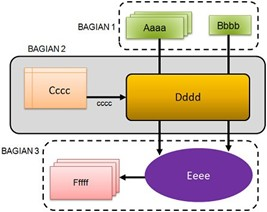
\includegraphics[width=0.8\textwidth]{assets/gambar_desain_sistem.jpeg}
  \caption{Arsitektur High-Level Sistem ADMA}
  \label{fig:arsitektur_high_level}
\end{figure}

Sistem terdiri dari tiga entitas utama yang saling berinteraksi secara asinkron:
\begin{enumerate}[label=\arabic*., leftmargin=*]
  \item \textbf{Go Binary (Agent)}\\
  Berjalan secara lokal pada setiap server target yang menjalankan backend FoodLAB. Bertanggung jawab mengumpulkan data telemetri, mengeksekusi instruksi dari control plane, dan menjalankan perintah lokal untuk diagnosis awal.
  
  \item \textbf{NATS Message Broker}\\
  Menyediakan saluran komunikasi asinkron berkinerja tinggi antara Agent dan Control Plane. NATS memfasilitasi pengiriman metrik secara publish-subscribe dan pengiriman instruksi secara request-reply \cite{fernando2021designing}.
  
  \item \textbf{C\# Control Plane (Backend)}\\
  Pusat pengendali terpusat yang mengelola siklus hidup agen, mengkoordinasikan alur investigasi anomali, melakukan panggilan ke API LLM untuk reasoning, dan menyediakan REST API untuk dashboard frontend.
\end{enumerate}

\subsection{Alur Handshake dan Bootstrap Agent}

Sebelum agen dapat mengirimkan data telemetri ke control plane, harus dilakukan proses jabat tangan (handshake) dan bootstrap terlebih dahulu untuk mendaftarkan identitas agen dan mendapatkan token otorisasi. Proses handshake dirancang menggunakan alur pertukaran pesan request-reply melalui NATS. Alur handshake ditunjukkan pada Gambar~\ref{fig:alur_handshake}.

\begin{figure}[H]
  \centering
  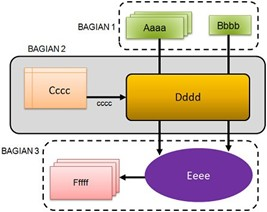
\includegraphics[width=0.8\textwidth]{assets/gambar_desain_sistem.jpeg}
  \caption{Alur Handshake dan Bootstrap Agent}
  \label{fig:alur_handshake}
\end{figure}

Langkah-langkah pada alur bootstrap adalah sebagai berikut:
\begin{enumerate}[label=\arabic*., leftmargin=*]
  \item Agen mengirimkan pesan registrasi (\texttt{RegisterAgentRequest}) yang memuat identitas host, alamat IP, sistem operasi, serta daftar container yang terpasang melalui subject \texttt{adma.registration}.
  \item Control plane menerima request tersebut, memverifikasi konfigurasi agen, menyimpan informasi agen ke database PostgreSQL, dan menghasilkan JWT (JSON Web Token) dengan scope terbatas sebagai token otorisasi.
  \item Control plane mengirimkan respons (\texttt{RegisterAgentResponse}) berisi token otorisasi dan konfigurasi pemantauan (seperti interval scraping metrik dan pola ekspresi reguler untuk pemindaian log) ke agen.
  \item Setelah menerima respons sukses, agen memasuki status aktif (\texttt{Active}) dan memulai routine worker untuk pemantauan.
\end{enumerate}

\subsection{Arsitektur Perception Agents}

Perception Layer dalam Go Binary terdiri dari tiga sub-agent spesialis yang berjalan sebagai goroutine independen secara konkuren. Struktur Perception Agents ditunjukkan pada Gambar~\ref{fig:arsitektur_perception}.

\begin{figure}[H]
  \centering
  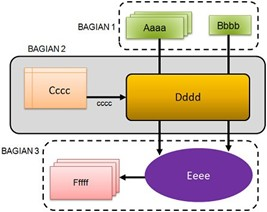
\includegraphics[width=0.8\textwidth]{assets/gambar_desain_sistem.jpeg}
  \caption{Arsitektur Perception Agents}
  \label{fig:arsitektur_perception}
\end{figure}

Tiga tipe Perception Agent utama didefinisikan sebagai berikut:
\begin{enumerate}[label=\arabic*., leftmargin=*]
  \item \textbf{Metric Perception Agent (MPA)}\\
  Terhubung ke database PostgreSQL menggunakan library driver sql dan mengeksekusi kueri ke view sistem \texttt{pg\_stat\_activity} pada interval yang ditentukan (default: 5 detik). MPA menyaring dan melaporkan koneksi aktif yang memiliki durasi eksekusi kueri melebihi ambang batas waktu tertentu (slow queries) serta query locking.
  
  \item \textbf{Log Perception Agent (LPA)}\\
  Menggunakan Docker SDK untuk membuat stream log yang berkelanjutan dari container backend yang dipantau. LPA memindai setiap baris log baru menggunakan pustaka ekspresi reguler (regex) untuk mendeteksi kata kunci error (seperti ``Exception'', ``Fatal'', ``Error'', ``Timeout''). Ketika kecocokan ditemukan, LPA mengemas log tersebut beserta metadata container (nama container, ID, timestamp) ke dalam log event terstruktur.
  
  \item \textbf{System Resource Agent (SRA)}\\
  Memantau penggunaan resource fisik pada level host dan container menggunakan gopsutil dan Docker Stats API. SRA melacak utilisasi CPU (dalam persen), konsumsi memori (dalam byte), utilisasi penyimpanan (disk I/O), dan status network interface.
\end{enumerate}

\subsection{Alur Kerja Reasoning Engine (RCA Pipeline)}

Reasoning Engine merupakan komponen paling kritis yang berada di dalam C\# Control Plane. Alur kerja Reasoning Engine menggunakan pendekatan Root Cause Analysis (RCA) Pipeline berbasis LLM. Alur kerja Reasoning Engine ditunjukkan pada Gambar~\ref{fig:alur_reasoning}.

\begin{figure}[H]
  \centering
  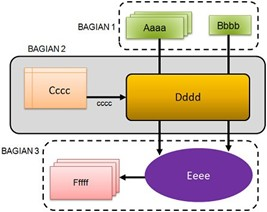
\includegraphics[width=0.8\textwidth]{assets/gambar_desain_sistem.jpeg}
  \caption{Alur Kerja Reasoning Engine (RCA Pipeline)}
  \label{fig:alur_reasoning}
\end{figure}

RCA Pipeline memproses data anomali melalui empat tahapan utama:
\begin{enumerate}[label=\arabic*., leftmargin=*]
  \item \textbf{Alert Correlator dan Pre-Filter}\\
  Menerima aliran data telemetri dari agen melalui sub-agent NATS. Alert Correlator mengelompokkan event yang terjadi pada jendela waktu yang sama (default: 30 detik) dan komponen yang berhubungan. Pre-Filter menyaring anomali berdasarkan aturan deterministik (seperti threshold CPU > 90\% atau kemunculan log kritis) untuk menentukan apakah diperlukan analisis LLM tingkat lanjut. Langkah ini penting untuk meminimalkan latensi dan konsumsi API LLM.
  
  \item \textbf{Context Enrichment}\\
  Jika Pre-Filter meloloskan insiden untuk diinvestigasi, control plane mengirimkan request ke agen target untuk mengumpulkan konteks tambahan. Konteks ini mencakup output perintah diagnostik (seperti \texttt{df -h}, \texttt{free -m}, daftar proses teratas via \texttt{top}, atau snapshot query database terakhir). Data enrichment ini digabungkan dengan alert history sebelumnya.
  
  \item \textbf{LLM Reasoning (Chain of Thought)}\\
  Data telemetri yang telah diperkaya dikemas ke dalam prompt terstruktur. Prompt ini dikirim ke API LLM (seperti Claude atau Gemini) menggunakan teknik Chain of Thought (CoT). LLM diminta melakukan diagnosis bertahap: (a) mendeskripsikan gejala sistem, (b) mengidentifikasi akar penyebab yang paling mungkin, (c) menghitung tingkat keyakinan diagnosis (\texttt{ValidityScore} dari 0--100), dan (d) menyusun rekomendasi tindakan remediasi beserta estimasi risiko aksi.
  
  \item \textbf{Validity Verification}\\
  Jika \texttt{ValidityScore} berada di atas ambang batas (default: 70), rencana aksi dilanjutkan ke alur eksekusi. Namun jika \texttt{ValidityScore} rendah, control plane menginstruksikan agen untuk menjalankan perintah diagnostik yang lebih spesifik berdasarkan saran dari model, mengulang pipeline investigasi sebelum keputusan akhir diambil.
\end{enumerate}

\subsection{Clean Architecture Backend ADMA}

Backend Control Plane dibangun dengan mengikuti prinsip Clean Architecture untuk memastikan kode terstruktur, modular, dan mudah diuji secara independen dari framework web maupun database. Pembagian layer ditunjukkan pada Gambar~\ref{fig:clean_architecture}.

\begin{figure}[H]
  \centering
  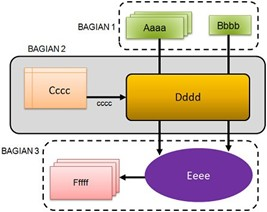
\includegraphics[width=0.8\textwidth]{assets/gambar_desain_sistem.jpeg}
  \caption{Clean Architecture Backend ADMA}
  \label{fig:clean_architecture}
\end{figure}

Desain layer backend ADMA \cite{valiveti2025evolution} terdiri dari:
\begin{enumerate}[label=\arabic*., leftmargin=*]
  \item \textbf{Domain Layer}\\
  Berisi entitas bisnis inti (seperti \texttt{Agent}, \texttt{Incident}, \texttt{RemediationAction}, \texttt{AuditLog}), value objects, domain events, dan antarmuka repository. Layer ini tidak memiliki dependensi ke library atau framework eksternal apa pun.
  
  \item \textbf{Application Layer}\\
  Berisi logika bisnis utama dan use case aplikasi (seperti \texttt{RegisterAgentCommandHandler}, \texttt{AnalyzeIncidentQueryHandler}, \texttt{ExecuteRemediationJob}). Layer ini mendefinisikan DTO (Data Transfer Objects) dan hanya bergantung pada Domain Layer.
  
  \item \textbf{Infrastructure Layer}\\
  Mengimplementasikan antarmuka yang didefinisikan di layer Domain dan Application. Layer ini mengintegrasikan Entity Framework Core untuk akses PostgreSQL, \texttt{NATS.Net} untuk komunikasi NATS, \texttt{AdmaNatsService} sebagai background service yang terus mendengarkan pesan dari agen, serta client API untuk integrasi ke Large Language Models (LLM).
  
  \item \textbf{API (Presentation) Layer}\\
  Sebagai entri point eksternal, mengimplementasikan ASP.NET Core Web API controller untuk mengekspos REST API dan SignalR Hub untuk push update data ke frontend dashboard.
\end{enumerate}

\subsection{Alur Deteksi Anomali dan Self-Healing}

Integrasi antara modul deteksi anomali di sisi agen, alur reasoning di control plane, dan eksekusi remediasi membentuk control loop self-healing yang otonom. Alur end-to-end penanganan insiden digambarkan pada Gambar~\ref{fig:alur_self_healing}.

\begin{figure}[H]
  \centering
  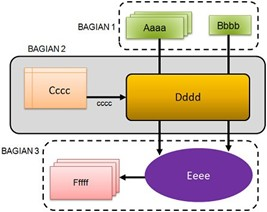
\includegraphics[width=0.8\textwidth]{assets/gambar_desain_sistem.jpeg}
  \caption{Alur Deteksi Anomali dan Self-Healing}
  \label{fig:alur_self_healing}
\end{figure}

Alur tersebut terdiri dari urutan proses berikut:
\begin{enumerate}[label=\arabic*., leftmargin=*]
  \item \textbf{Detection}: Log Perception Agent pada Go binary mendeteksi log pengecualian kritis (\texttt{Exception}) berulang pada container backend C\# ASP.NET Core FoodLAB. Sinyal dikirim via NATS ke Control Plane.
  \item \textbf{Ingestion}: Control plane menangkap event, membuat entitas \texttt{Incident} baru dengan status \texttt{Triggered}, dan mengaktifkan alert correlator.
  \item \textbf{Analysis}: Reasoning Engine melakukan call LLM dengan CoT, mendiagnosa bahwa database PostgreSQL mengalami connection pool exhaustion karena ada query locking yang tidak dilepaskan. LLM menghasilkan rencana tindakan: (a) Kill query pengunci di database PostgreSQL, (b) Restart container backend FoodLAB untuk me-reset connection pool.
  \item \textbf{Risk Assessment}: LLM mendeteksi bahwa restart container memiliki tingkat risiko sedang (dapat menyebabkan interupsi request sesaat), sedangkan kill query memiliki tingkat risiko rendah.
  \item \textbf{Execution}: Untuk tindakan berisiko sedang, sistem mengirimkan notifikasi persetujuan ke dashboard operator. Setelah operator menyetujui (atau otomatis disetujui jika mode full-autonomous diaktifkan), control plane mengirimkan perintah \texttt{KillQuery} dan \texttt{RestartContainer} via NATS ke agen.
  \item \textbf{Verification}: Agen mengeksekusi perintah tersebut, memverifikasi status container kembali menjadi \texttt{Running}, dan memantau metrik koneksi database selama 60 detik. Setelah memastikan sistem stabil, status incident diperbarui menjadi \texttt{Resolved}.
\end{enumerate}

\subsection{Alur Kerja Code Fix Agent}

Apabila Reasoning Engine mendiagnosa bahwa akar penyebab anomali berasal dari bug di level kode sumber aplikasi (misalnya kegagalan penanganan null value, syntax error pada query database, atau kebocoran memori pada class tertentu), sistem mengaktifkan sub-flow Code Fix Agent. Alur kerja Code Fix Agent ditunjukkan pada Gambar~\ref{fig:alur_code_fix}.

\begin{figure}[H]
  \centering
  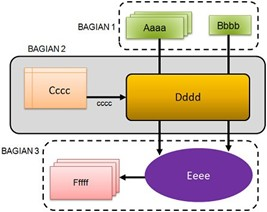
\includegraphics[width=0.8\textwidth]{assets/gambar_desain_sistem.jpeg}
  \caption{Alur Kerja Code Fix Agent}
  \label{fig:alur_code_fix}
\end{figure}

Mekanisme kerja Code Fix Agent dirancang sebagai berikut:
\begin{enumerate}[label=\arabic*., leftmargin=*]
  \item \textbf{Code Retrieval}: Control plane menggunakan REST API GitLab untuk mengambil file kode sumber yang diidentifikasi oleh LLM memiliki bug (misalnya file controller C\# atau model C\#).
  \item \textbf{Patch Generation}: Code Fix Agent mengirimkan kode sumber tersebut beserta log error dan diagnosis LLM ke model LLM spesialis pengkodean untuk menghasilkan perbaikan kode berupa file diff (patch).
  \item \textbf{Local Validation}: Agen melakukan kompilasi lokal menggunakan toolchain C\# SDK dan menjalankan unit test yang ada pada code base untuk memastikan bahwa perubahan yang diusulkan tidak merusak fungsionalitas lain (regression test).
  \item \textbf{Merge Request Submission}: Setelah validasi lokal berhasil, Code Fix Agent membuat git branch baru, melakukan commit perubahan dengan format conventional commits, melakukan push ke GitLab remote, dan membuat Merge Request (MR) ke target branch utama dengan menyertakan tautan log incident sebagai referensi.
  \item \textbf{Operator Notification}: Operator mendapat notifikasi pada dashboard tentang adanya MR perbaikan otomatis yang siap ditinjau dan digabungkan.
\end{enumerate}

\subsection{Desain Antarmuka Dashboard Operator}

Dashboard operator dirancang sebagai Single Page Application (SPA) berbasis React \cite{barros2023examining} untuk memberikan visualisasi real-time terhadap status operasional backend FoodLAB dan aktivitas framework ADMA. Desain antarmuka dashboard operator ditunjukkan pada Gambar~\ref{fig:desain_dashboard}.

\begin{figure}[H]
  \centering
  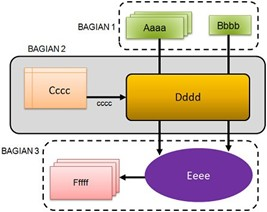
\includegraphics[width=0.8\textwidth]{assets/gambar_desain_sistem.jpeg}
  \caption{Desain Antarmuka Dashboard Operator}
  \label{fig:desain_dashboard}
\end{figure}

Desain antarmuka dashboard memiliki beberapa bagian utama:
\begin{enumerate}[label=\arabic*., leftmargin=*]
  \item \textbf{Navigation Bar}: Menu navigasi untuk beralih antara halaman Dashboard utama, Agent List, Incident Log, Remediation History, dan Settings.
  \item \textbf{System Status Metrics}: Menampilkan indikator performa utama (KPI) secara real-time seperti total Active Agents, CPU/Memory Host, rata-rata MTTR, dan jumlah incident dengan status active.
  \item \textbf{Agent Status Grid}: Kartu visual untuk setiap agen yang terdaftar. Menampilkan status koneksi agen (Online/Offline), versi agent, utilisasi CPU/Memory container utama, dan status kesehatan container.
  \item \textbf{Real-time Incident Alert Panel}: Panel samping yang menampilkan daftar incident yang sedang aktif. Panel ini menampilkan status severity (Low, Medium, High, Critical) dengan animasi berdenyut untuk menarik perhatian operator. Mengklik kartu incident akan membuka modal detail yang berisi: (a) diagnosis akar masalah hasil reasoning LLM, (b) data telemetri pendukung (error log snippet dan grafik metrik), dan (c) rencana aksi remediasi yang diusulkan beserta tombol persetujuan (\texttt{Approve/Reject}).
  \item \textbf{Audit Trail Log}: Menampilkan riwayat log aktivitas yang komprehensif, mencatat setiap deteksi anomali, panggilan LLM, persetujuan operator, dan hasil eksekusi tindakan remediasi untuk kebutuhan audit kepatuhan sistem.
\end{enumerate}

Antarmuka ini diimplementasikan menggunakan arsitektur komponen React yang modular, memanfaatkan TanStack Query untuk server-side state synchronization, SignalR Client untuk push event real-time, dan Tailwind CSS untuk styling yang responsif pada berbagai ukuran layar. Autentikasi ke dashboard diamankan melalui integrasi Keycloak SSO \cite{thorgersen2023keycloak}.